\documentclass[t,12pt,numbers,fleqn]{beamer}
%\documentclass[t,12pt,numbers,fleqn,handout]{beamer}

\usepackage{latexsym}
\usepackage{amssymb}
\usepackage{stmaryrd}
\usepackage{phonetic}
\usepackage{wasysym}
\usepackage{pgf}
\usepackage{tikz}
\usepackage{url}
\usetikzlibrary{arrows}
\usepackage{array}
\usepackage{pgfpages} 
\usepackage{multirow} 
\usepackage{graphicx}
\usepackage{color}
\usepackage{listings}
\usepackage{hyperref}
\hypersetup{colorlinks=true,
    linkcolor=blue,
    citecolor=blue,
    filecolor=blue,
    urlcolor=blue,
    unicode=false}

\lstset{language=lisp,basicstyle=\ttfamily,breaklines=true,showspaces=false,showstringspaces=false,breakatwhitespace=true,texcl=true,escapeinside={\%*}{*)}}

%\pgfpagesuselayout{resize to}[letterpaper, border shrink=5mm,landscape] 
%\pgfpagesuselayout{2 on 1}[letterpaper,border shrink=5mm] 

\usepackage{fancybox}
%\usepackage{times}

\useoutertheme{split}

\mode<presentation>{}

%\mode<presentation>{
%\usecolortheme{whale}
%\usecolortheme{orchid}
%\useinnertheme[shadow]{rounded}
%}

%\setbeamerfont{structure}{series=\bfseries}
%\usefonttheme[stillsansseriftext,stillsansserifmath]{serif}
%\usetheme{Madrid}

\setbeamertemplate{navigation symbols}{} 
\setbeamertemplate{itemize item}[ball]
\setbeamersize{text margin left = 4mm}
\setbeamersize{text margin right = 4mm}

%% Requires:
%% 
%% \usepackage{latexsym}
%% \usepackage{amssymb}
%% \usepackage{stmaryrd}

%\renewcommand{\labelenumi}{(\theenumi)}
\newcommand{\be}{\begin{enumerate}}
\newcommand{\ee}{\end{enumerate}}
\newcommand{\bi}{\begin{itemize}}
\newcommand{\ei}{\end{itemize}}
\newcommand{\bc}{\begin{center}}
\newcommand{\ec}{\end{center}}
\newcommand{\bsp}{\begin{sloppypar}}
\newcommand{\esp}{\end{sloppypar}}

\newcommand{\sglsp}{\ }
\newcommand{\dblsp}{\ \ }

\newcommand{\iclicker}{i\texttt{>}clicker}

\newcommand{\sA}{\mbox{$\cal A$}}
\newcommand{\sB}{\mbox{$\cal B$}}
\newcommand{\sC}{\mbox{$\cal C$}}
\newcommand{\sD}{\mbox{$\cal D$}}
\newcommand{\sE}{\mbox{$\cal E$}}
\newcommand{\sF}{\mbox{$\cal F$}}
\newcommand{\sG}{\mbox{$\cal G$}}
\newcommand{\sH}{\mbox{$\cal H$}}
\newcommand{\sI}{\mbox{$\cal I$}}
\newcommand{\sJ}{\mbox{$\cal J$}}
\newcommand{\sK}{\mbox{$\cal K$}}
\newcommand{\sL}{\mbox{$\cal L$}}
\newcommand{\sM}{\mbox{$\cal M$}}
\newcommand{\sN}{\mbox{$\cal N$}}
\newcommand{\sO}{\mbox{$\cal O$}}
\newcommand{\sP}{\mbox{$\cal P$}}
\newcommand{\sQ}{\mbox{$\cal Q$}}
\newcommand{\sR}{\mbox{$\cal R$}}
\newcommand{\sS}{\mbox{$\cal S$}}
\newcommand{\sT}{\mbox{$\cal T$}}
\newcommand{\sU}{\mbox{$\cal U$}}
\newcommand{\sV}{\mbox{$\cal V$}}
\newcommand{\sW}{\mbox{$\cal W$}}
\newcommand{\sX}{\mbox{$\cal X$}}
\newcommand{\sY}{\mbox{$\cal Y$}}
\newcommand{\sZ}{\mbox{$\cal Z$}}

\renewcommand{\phi}{\varphi}
\newcommand{\seq}[1]{{\langle #1 \rangle}}
\newcommand{\set}[1]{{\{ #1 \}}}
\newcommand{\tuple}[1]{{( #1 )}}
\newcommand{\mlist}[1]{{[ #1 ]}}
\newcommand{\sembrack}[1]{\llbracket#1\rrbracket}
\newcommand{\redsembrack}[1]{\bred{\llbracket}#1\bred{\rrbracket}}
%\newcommand{\sembrack}[1]{[\![#1]\!]}
\newcommand{\synbrack}[1]{\ulcorner#1\urcorner}
\newcommand{\commabrack}[1]{\lfloor#1\rfloor}
\newcommand{\bsynbrack}[1]{\lceil#1\rceil}
\newcommand{\bsembrack}[1]{\lceil\!\!\lceil#1\rceil\!\!\rceil}
\newcommand{\mname}[1]{\mbox{\sf #1}}
\newcommand{\mcolon}{\mathrel:}
\newcommand{\mdot}{\mathrel.}
\newcommand{\modpar}{\models_{\rm par}}
\newcommand{\modreg}{\models_{\rm reg}}
\newcommand{\proves}[2]{#1 \vdash #2}
\newcommand{\notproves}[2]{#1 \not\vdash #2}
\newcommand{\provesin}[3]{#1 \vdash_{#2} #3}
\newcommand{\notprovesin}[3]{#1 \not\vdash_{#2} #3}
%\newcommand{\leqq}[1]{\mathrel{\preceq_{#1}}}
\newcommand{\parrow}{\rightharpoonup}
\newcommand{\tarrow}{\rightarrow}
\newcommand{\term}{\seq}
\newcommand{\lub}{\sqcup}
\newcommand{\subfun}{\sqsubseteq}
\newcommand{\subpred}{\subseteq}
\newcommand{\BoxApp}{\Box\,}
\newcommand{\BOX}{\mathrel{\Box}}
\newcommand{\funapp}{\mathrel@}

\newcommand{\com}{\mname{complement}}
\newcommand{\dom}{\mname{domain}}
\newcommand{\sumcl}{\mname{sum}}
\newcommand{\pow}{\mname{power}}
\newcommand{\pair}{\mname{pair}}
\newcommand{\opair}{\mname{ordered-pair}}
\newcommand{\inters}{\mname{intersection}}
\newcommand{\emp}{\mname{empty}}
\newcommand{\uni}{\mname{univocal}}
\newcommand{\fun}{\mname{function}}
\newcommand{\card}{\mname{card}}
\newcommand{\sets}{\mname{sets}}
\newcommand{\monotone}{\mname{monotone}}
\newcommand{\continuous}{\mname{continuous}}
\newcommand{\chain}{\mname{chain}}
\newcommand{\mub}{\mname{ub}}
\newcommand{\mlub}{\mname{lub}}
\newcommand{\fixedpoint}{\mname{fp}}
\newcommand{\leastfixedpoint}{\mname{lfp}}
\newcommand{\strongfixedpoint}{\mname{sfp}}
\newcommand{\emptyfun}{\triangle}
\newcommand{\statetrans}[1]{\stackrel{#1}{\longrightarrow}}
\newcommand{\thyext}{\leq}
\newcommand{\conthyext}{\unlhd}

\newcommand{\Iota}{\mbox{\rm I}}
\newcommand{\IotaApp}{\mbox{\rm I}\,}
\newcommand{\iotaApp}{\iota\,}
\newcommand{\epsilonApp}{\epsilon\,}
%\newcommand{\True}{\mbox{\sf T}} 
%\newcommand{\False}{\mbox{\sf F}} 
\newcommand{\Trueword}{\sf true}
\newcommand{\Falseword}{\sf false}
\newcommand{\Neg}{\neg} 
\newcommand{\Andd}{\wedge}
%\newcommand{\Or}{\vee}
\newcommand{\Orr}{\vee}
\newcommand{\Implies}{\supset}
\newcommand{\ImpliesAlt}{\Rightarrow}
\newcommand{\Iff}{\equiv}
\newcommand{\Sheffer}{\mathrel|}
\newcommand{\IffAlt}{\Leftrightarrow}
\newcommand{\Forall}{\forall}
\newcommand{\ForallApp}{\forall\,}
\newcommand{\Forsome}{\exists}
\newcommand{\ForsomeApp}{\exists\,}
\newcommand{\ForsomeUniqueApp}{\exists\,!\,}
\newcommand{\IsDef}{\downarrow}
\newcommand{\IsUndef}{\uparrow}
\newcommand{\Equal}{=}
\newcommand{\QuasiEqual}{\simeq}
\newcommand{\Undefined}{\bot}
\newcommand{\If}{\mname{if}}
\newcommand{\IsDefApp}{\!\IsDef}
\newcommand{\IsUndefApp}{\!\IsUndef}
\newcommand{\TRUE}{\mbox{{\sc t}}}
\newcommand{\FALSE}{\mbox{{\sc f}}}
\newcommand{\truthvalues}{\{\TRUE,\FALSE\}}
\newcommand{\LambdaApp}{\lambda\,}
\newcommand{\LAMBDAapp}{\Lambda\,}
\newcommand{\PiApp}{\Pi\,}
\newcommand{\SigmaApp}{\Sigma\,}
\newcommand{\AlphaEquiv}{\stackrel{\alpha}{=}}

\newcommand{\mvar}[3]{\textbf{var}_{#1}[#2,#3]}
\newcommand{\mterm}[2]{\textbf{term}_{#1}[#2]}
\newcommand{\mform}[2]{\textbf{form}_{#1}[#2]}
\newcommand{\mtype}[2]{\textbf{type}_{#1}[#2]}
\newcommand{\mexpr}[3]{\textbf{expr}_{#1}[#2,#3]}

\newcommand{\imps}{\mbox{\sc imps}}
\newcommand{\fol}{\mbox{\sc fol}}
\newcommand{\pf}{${\bf PF}$}
\newcommand{\pfstar}{${\bf PF}^\ast$}
\newcommand{\lutins}{\mbox{\sc lutins}}
\newcommand{\vlisp}{\mbox{\sc vlisp}}
\newcommand{\vmach}{\mbox{\sc vmach}}
\newcommand{\gnu}{\mbox{\sc gnu}}
\newcommand{\zf}{\mbox{\sc zf}}
\newcommand{\nbg}{\mbox{\sc nbg}}
\newcommand{\pnbg}{\mbox{\sc pnbg}}
\newcommand{\snbg}{\mbox{\sc snbg}}
\newcommand{\pfol}{\mbox{\sc pfol}}
\newcommand{\nbgstar}{$\mbox{\sc nbg}^\ast$}
\newcommand{\boldnbgstar}{$\mbox{\bf NBG}^\ast$}
\newcommand{\stt}{\mbox{\sc stt}}
\newcommand{\eves}{\mbox{\sc eves}}
\newcommand{\hol}{\mbox{\sc hol}}
\newcommand{\mizar}{Mizar}
\newcommand{\nqthm}{Nqthm}
\newcommand{\pvs}{\mbox{\sc pvs}}
\newcommand{\stmm}{\mbox{\sc stmm}}

\iffalse
\newtheorem{thm}{Theorem}[section]
\newtheorem{cor}[thm]{Corollary}
\newtheorem{lem}[thm]{Lemma}
\newtheorem{prop}[thm]{Proposition}
\newtheorem{rem}[thm]{Remark}
\newtheorem{eg}[thm]{Example}
\newtheorem{df}[thm]{Definition}
\fi

%\newenvironment{proof}{\par\noindent{\bf Proof\ \ }}{$\Box$}

\newenvironment{namedform}[1]
   {\begin{tabbing}\textbf{#1}\ }
   {\end{tabbing}}

\newcommand{\urlpart}[1]{\mbox{\texttt{#1}}\linebreak[0]}

\newcommand{\bblue}{\textcolor{blue!80!black}}
\newcommand{\bgreen}{\textcolor{green!55!black}}
\newcommand{\bbrown}{\textcolor{brown}}
\newcommand{\bred}{\textcolor{red!80!black}}
\newcommand{\bcyan}{\textcolor{cyan!80!black}}
\newcommand{\bmagenta}{\textcolor{magenta}}
\newcommand{\byellow}{\textcolor{yellow}}
\newcommand{\borange}{\textcolor{orange}}
\newcommand{\bviolet}{\textcolor{violet}}
\newcommand{\bpurple}{\textcolor{purple}}
\newcommand{\bdarkgray}{\textcolor{darkgray}}
\newcommand{\bgray}{\textcolor{gray}}
\newcommand{\blightgray}{\textcolor{lightgray}}

\newcommand{\clicker}{i\texttt{>}clicker}

\newenvironment{changemargin}[2]{%
  \begin{list}{}{%
    \setlength{\topsep}{0pt}%
    \setlength{\leftmargin}{#1}%
    \setlength{\rightmargin}{#2}%
    \setlength{\listparindent}{\parindent}%
    \setlength{\itemindent}{\parindent}%
    \setlength{\parsep}{\parskip}%
  }%
  \item[]}{\end{list}}
%$

\newcommand{\qzero}{${\cal Q}_0$}
\newcommand{\qzerou}{${\cal Q}^{\rm u}_{0}$}
\newcommand{\qzerouqe}{${\cal Q}^{\rm uqe}_{0}$}
\newcommand{\churchqe}{$\mbox{\sc ctt}_{\rm qe}$}
\newcommand{\churchuqe}{$\mbox{\sc ctt}_{\rm uqe}$}
\newcommand{\NegAlt}{{\sim}}
\newcommand{\wff}[1]{{\sf wff}_{#1}}
\newcommand{\additionu}[1]{\textcolor{blue}{#1}}
\newcommand{\additionuqe}[1]{\textcolor{red}{#1}}

\newcommand{\high}{\bred{\rotatebox[origin=c]{90}{\CIRCLE}}}
\newcommand{\medhigh}{\bred{\rotatebox[origin=c]{90}{\RIGHTcircle}}}
\newcommand{\medlow}{\bred{\rotatebox[origin=c]{-90}{\RIGHTcircle}}}
\newcommand{\low}{\bred{\rotatebox[origin=c]{90}{\Circle}}}


\title{ {\normalsize \bgreen{\bf CICM 2018}}\\[1.5ex]
  {\large \bf Biform Theories: Project Description}
\vspace{-1.5ex}
}

\author[Farmer]{
Jacques Carette, \underline{William M. Farmer}, and Yasmine Sharoda
\vspace*{-0.5ex}
}

\institute{
Department of Computing and Software\\
McMaster University
\vspace*{-1.5ex}
} 

\date{
{\small 16 August 2018}

\bc
 \includegraphics[scale = 0.2, keepaspectratio]
{$HOME/doc/images/mcmaster-logo-full-color.jpg}%$
\ec
}

\begin{document}

%%%%%%%%%%%%%%%%%%%%%%%%%%%%%%%%%%%%%%%%%%%%%%%%%%%%%%%%%%%%

\setbeamertemplate{footline}{}
\begin{frame}
\vspace{-1.5ex} 
\titlepage
\end{frame}

\setbeamertemplate{footline}{
\begin{beamercolorbox}{sectioninhead/foot}
\bblue{\hrulefill}

\vspace{1ex}
\hspace{1ex}
{\tiny Carette, Farmer, Sharoda
\hfill 
Biform Theories: Project Description
\hfill
\insertframenumber/\ref{lastframe}}
\vspace{1ex}
\end{beamercolorbox}}

%%%%%%%%%%%%%%%%%%%%%%%%%%%%%%%%%%%%%%%%%%%%%%%%%%%%%%%%%%%%

\begin{frame}
\frametitle{Outline}
\bi

  \item Motivation.

  \item Notion of a biform theory.

  \item Project objectives.

  \item Project status.

\ei
\end{frame}

%%%%%%%%%%%%%%%%%%%%%%%%%%%%%%%%%%%%%%%%%%%%%%%%%%%%%%%%%%%%

\begin{frame}
\frametitle{Semantics  vs.~Syntax}
\bi

  \item Consider the mathematical expression 

  \bi

    \item[] $(x + 2) * (2 * x + 1) + 3 * x$

  \ei

  where $x$ denotes a natural number.

\pause

  \item This expression $e$ has two values:

  \be

\pause

    \item A \bblue{semantic value} that is
      the natural number denoted by $e$.

\pause

    \item A \bblue{syntactic value} that is the expression $e$ itself
      having the form of a polynomial (which we denote by the
      quotation $\bluesynbrack{e}$).

  \ee

\pause

  \item Some operations apply to semantic values.

  \bi

    \item \bbrown{Examples}: \bgreen{$+$} and \bgreen{$*$}.

  \ei

  \item Other operations apply to syntactic values.

  \bi

    \item \bbrown{Examples}: \bgreen{normalize} and \bgreen{factor}.

  \ei


\ei
\end{frame}

%%%%%%%%%%%%%%%%%%%%%%%%%%%%%%%%%%%%%%%%%%%%%%%%%%%%%%%%%%%%

\begin{frame}
\frametitle{Transformers}
\bi

  \item Let $\sE$ be a set of expressions.

  \item A \bblue{transformer} is an algorithm that implements a
    function $\sE^n \tarrow \sE$.

  \bi

    \item \bbrown{Examples}: normalize and factor.

  \ei

\pause

  \item Operations on semantic values can often be computed by
    transformers.

\bc
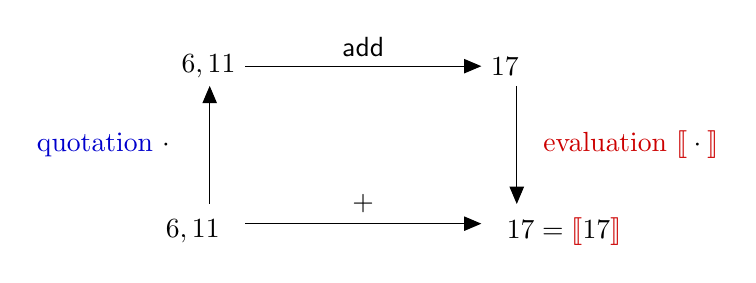
\begin{tikzpicture}[scale=0.5]
\draw[-triangle 45] (-3,2) -- (+3,2);
  \draw[left] (-3,2) node {$\bluesynbrack{6},\bluesynbrack{11}$};
  \draw[right] (+3,2) node {$\bluesynbrack{17}$};
  \draw[] (0,2.5) node {$\mname{add}$};
\draw[-triangle 45] (-3,-2) -- (+3,-2);
  \draw[left] (-3.4,-2.2) node {$6,11$};
  \draw[right] (+3.4,-2.2) node {$17 = \redsembrack{\bluesynbrack{17}}$};
  \draw[] (0,-1.5) node {$+$};
\draw[-triangle 45] (+3.9,+1.5) -- (+3.9,-1.5);
  \draw[] (-6.6,0) node {\bblue{quotation} $\bluesynbrack{\cdot}$};
\draw[-triangle 45] (-3.9,-1.5) -- (-3.9,+1.5);
  \draw[] (+6.8,0) node {\bred{evaluation} $\redsembrack{\cdot}$};
\end{tikzpicture}
\ec

\item Note: The two operators are related by the \bblue{law of disquotation}:

  \bi

    \item[] $\redsembrack{\bluesynbrack{e}} = e$.

  \ei

\ei
\end{frame}

%%%%%%%%%%%%%%%%%%%%%%%%%%%%%%%%%%%%%%%%%%%%%%%%%%%%%%%%%%%%

\begin{frame}
\frametitle{Syntax-Based Mathematical Algorithms}
\bi

  \item A \bblue{syntax-based mathematical algorithm (SBMA)}
    \bbrown{[Far13]} is an transformer that manipulates the syntax of
    mathematical expressions in a mathematically meaningful way.

  \bi

    \item \bbrown{Examples}: normalize, factor, add.

  \ei

\pause

  \item \bred{SBMAs are commonplace in mathematics!}

\pause

  \item A SBMA $A$ has two fundamental properties:

  \be

    \item The \bblue{computational behavior} of $A$ is the relationship
    between the input and output expressions of $A$.

    \item The \bblue{mathematical meaning} of $A$ is the relationship
      between what the input and output expressions of $A$ mean
      mathematically.

  \ee

  \item A \bblue{meaning formula} for $A$ is a statement that
    expresses the mathematical meaning of $A$.

\ei
\end{frame}

%%%%%%%%%%%%%%%%%%%%%%%%%%%%%%%%%%%%%%%%%%%%%%%%%%%%%%%%%%%%

\begin{frame}
\frametitle{Examples of Meaning Formulas}
\bi

  \item The meaning formula for \mname{add} is:

  \bi

    \item[] \only<1>{$\ForallApp x,y : \mname{Numeral} \mdot
      \mname{add}(x,y) = x + y$.}

    \only<2->{$\ForallApp x,y : \mname{Numeral} \mdot
    \redsembrack{\mname{add}(x,y)} = \redsembrack{x} + \redsembrack{y}$.}

  \ei

  \only<3->{An instance of the meaning formula is:

  \bi

    \item[] $\redsembrack{\mname{add}(\bluesynbrack{6},\bluesynbrack{11})} =
      \redsembrack{\bluesynbrack{6}} + \redsembrack{\bluesynbrack{11}}$

  \ei
  }

  \only<4->{
  \item The meaning formula for \mname{normalize} is:

  \bi

    \item[] $\ForallApp p,q \mcolon \mname{Poly} \mdot$\\
      \hspace{2ex}$(\ForallApp x \mcolon \mathbb{N} \mdot
      \redsembrack{p} = \redsembrack{\mname{normalize}(p)}) \Andd
                  {}$\\
      \hspace{2ex}$(\ForallApp x \mcolon \mathbb{N} \mdot
      \redsembrack{p} = \redsembrack{q}) \Iff \mname{normalize}(p) =
      \mname{normalize}(q)$

  \ei
  }

\ei
\end{frame}

%%%%%%%%%%%%%%%%%%%%%%%%%%%%%%%%%%%%%%%%%%%%%%%%%%%%%%%%%%%%

\begin{frame}
\frametitle{Axiomatic Theories vs.~Algorithmic Theories}
\bi

  \item Let $L$ be a language in some underlying logic.

  \item An \bblue{axiomatic theory} is a pair $T=(L,\Gamma)$ where
    $\Gamma$ is a set of formulas of $L$ that serve as the axioms of
    $T$.

  \bi

    \item Axiomatic theories are implemented in \bgreen{proof
      assistants}.

  \ei

\pause

  \item An \bblue{algorithmic theory} is a pair $(L,\Pi)$ where $\Pi$
    is is a set of transformers that implement functions on the
    expressions of $L$.

  \bi

    \item Algorithmic theories are implemented in \bgreen{computer
      algebra systems}.

  \ei

\pause

  \item \bblue{Problem}.  Can an axiomatic theory and algorithmic
    theory be combined so that we can define and reason about SBMAs in
    the same context?

\pause

  \item \bred{Our solution is the notion of a biform theory.}

\ei
\end{frame}

%%%%%%%%%%%%%%%%%%%%%%%%%%%%%%%%%%%%%%%%%%%%%%%%%%%%%%%%%%%%

\begin{frame}
\frametitle{Biform Theories}
\bi

  \item A \bblue{biform theory} is a triple $T=(L,\Pi,\Gamma)$ where:

  \be

    \item $L$ is a language of some underlying logic.

    \item $\Pi$ is a set of transformers that implement functions on
      the expressions of $L$.

    \item $\Gamma$ is a set of formulas of $L$ that serve as the axioms of $T$.

  \ee

  \item For each $\pi \in \Pi$, $L$ includes a name for the function
    implemented by $\pi$ that serves as a name for $\pi$.

  \item The axioms of $T$ specify the meaning of the nonlogical
    symbols of $L$ including the names of the transformers of $T$.

  \item The transformers may be written in $L$ or in a programming
    language external to $L$.

  \item $T$ is an axiomatic theory if $\Pi$ is empty and is an
    algorithmic theory if $\Gamma$ is empty.

\ei
\end{frame}

%%%%%%%%%%%%%%%%%%%%%%%%%%%%%%%%%%%%%%%%%%%%%%%%%%%%%%%%%%%%

\begin{frame}
\frametitle{Formalizing Biform Theories}
\bi

  \item To formalize a biform theory in a logic \textbf{Log} we need
    to be able to formalize SBMAs in \textbf{Log}.

\pause

  \item To formalize an SBMA $A$ in \textbf{Log} we must:

  \be

    \item Define or specify in \textbf{Log} a function $B$ on
      syntactic values representing $A$.

    \item State and prove in \textbf{Log} the meaning formula for
      $B$ from the definition or specification of $B$.

    \item Apply $B$ to mathematical expressions in \textbf{Log} by
      instantiating the meaning formula for $B$ and then applying the
      result.

  \ee

\ei
\end{frame}

%%%%%%%%%%%%%%%%%%%%%%%%%%%%%%%%%%%%%%%%%%%%%%%%%%%%%%%%%%%%

\begin{frame}
\frametitle{Standard Approach: Local Reflection}
\bi

  \item Let $A$ be an SBMA on expressions in a language $L_{\rm obj}$
    of some logic \textbf{Log}.

  \item We build a \bblue{metareasoning infrastructure} in
    \textbf{Log} consisting of:

  \be

    \item An \bgreen{inductive type} $L_{\rm syn}$ of syntactic values
      representing the expressions in $L_{\rm obj}$.

    \item A \bgreen{quotation operator} $\bluesynbrack{\cdot}$ mapping
      expressions in $L_{\rm obj}$ to syntactic values of $L_{\rm
        syn}$.

    \item An \bgreen{evaluation operator} $\redsembrack{\cdot}$
      mapping syntactic values of $L_{\rm syn}$ to values of $L_{\rm
        obj}$.

  \ee

  \item We define a function $B$ in \textbf{Log} from syntactic values
    representing inputs of $A$ to syntactic values representing
    outputs of $A$.

  \item The infrastructure is \bgreen{local} in the sense that $L_{\rm
    obj}$ is not the whole language $L$ of Log.

\ei
\end{frame}

%%%%%%%%%%%%%%%%%%%%%%%%%%%%%%%%%%%%%%%%%%%%%%%%%%%%%%%%%%%%

\begin{frame}
\frametitle{Local Reflection}
\vspace*{-3ex}
\vfill
\begin{figure}
\center
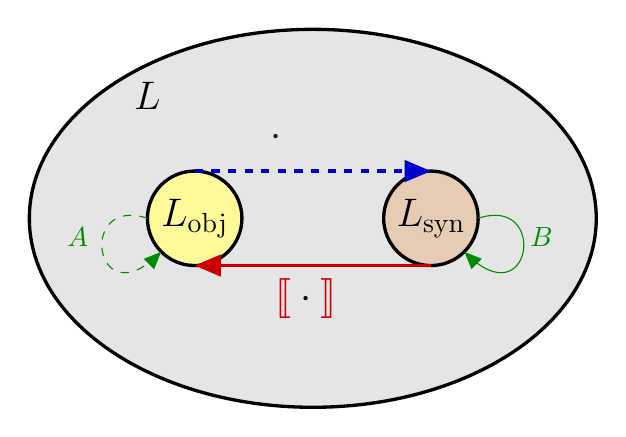
\begin{tikzpicture}[scale=.6]
  \filldraw[very thick, fill=gray!20] (3.5,0) ellipse (6 and 4);
    \draw (0,+2.6) node {\Large $L$};
  \filldraw[very thick, fill=yellow!40] (+1,0) circle (1);
    \draw (+1,0) node {\Large $L_{\rm obj}$};
  \filldraw[very thick, fill=brown!40] (+6,0) circle (1);
    \draw (+6,0) node {\Large $L_{\rm syn}$};
  \draw[-triangle 45, very thick, dashed, color=blue!80!black] (+1,+1) -- (+6,+1);
    \draw[right] (+2.4,+1.7) node {\Large $\bluesynbrack{\cdot}$};
  \draw[-triangle 45, very thick, color=red!80!black] (+6,-1) -- (+1,-1);
    \draw[right] (+2.5,-1.7) node {\Large $\redsembrack{\cdot}$};
  \draw[-triangle 45, dashed, color=green!55!black] (0,0) .. controls 
    (-1.5,.5) and (-1.13,-2.13) .. (.29,-.71);
    \draw[right] (-1.9,-.4) node {\bgreen{$A$}};
  \draw[-triangle 45, color=green!55!black] (7,0) .. controls 
    (8.5,.5) and (8.13,-2.13) .. (6.71,-.71);
    \draw[right] (7.9,-.4) node {\bgreen{$B$}};
\end{tikzpicture}
\end{figure}
\vfill
\end{frame}

%%%%%%%%%%%%%%%%%%%%%%%%%%%%%%%%%%%%%%%%%%%%%%%%%%%%%%%%%%%%

\begin{frame}
\frametitle{An Alternate Approach: Global Reflection}
\bi

  \item Local reflection does not scale up well:

  \bi

    \item Each collection of SBMAs requires a separate infrastructure.

    \item Extending an SBMA to a new domain requires a new
      infrastructure.

  \ei

  \item Global reflection employs a single infrastructure for all
    SBMAs:

  \be

    \item An \bgreen{inductive type} representing the entire set of expressions.

    \item A \bgreen{global quotation operator} $\bluesynbrack{\cdot}$.

    \item A \bgreen{global evaluation operator} $\redsembrack{\cdot}$.

  \ee

  \item Global reflection requires a logic with global quotation and
    evaluation operators.

  \item \bred{It is an open problem whether global reflection is
    viable!}

\iffalse
  \item To test the viability of global reflection, we want to
    incorporate global quotation and evaluation into a traditional
    logic.
\fi

\ei
\end{frame}

%%%%%%%%%%%%%%%%%%%%%%%%%%%%%%%%%%%%%%%%%%%%%%%%%%%%%%%%%%%%

\begin{frame}
\frametitle{Global Reflection}
\vspace*{-3ex}
\vfill
\begin{figure}
\center
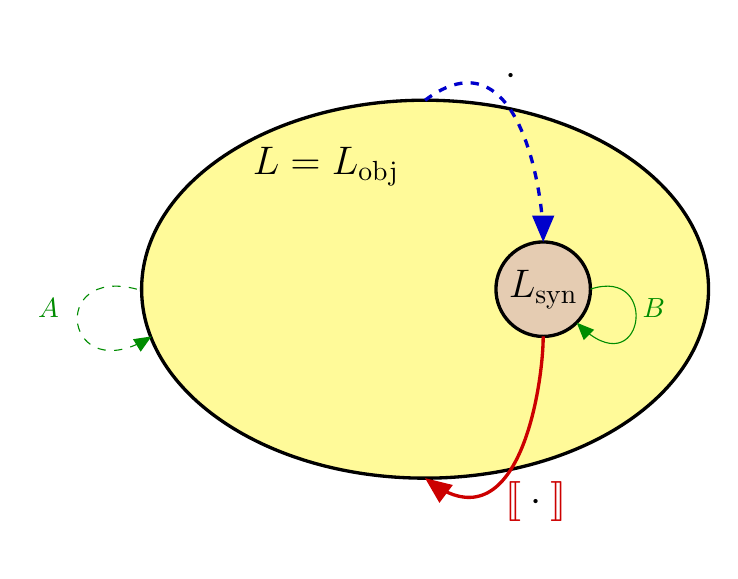
\begin{tikzpicture}[scale=.6]
  \filldraw[very thick, fill=yellow!40] (3.5,0) ellipse (6 and 4);
    \draw (+1.4,+2.6) node {\Large $L=L_{\rm obj}$};
  \filldraw[very thick, fill=brown!40] (+6,0) circle (1);
    \draw (+6,0) node {\Large $L_{\rm syn}$};
  \draw[-triangle 45, very thick, dashed, color=blue!80!black] (3.5,4) .. controls
    (5.5,5.5) and (6,2).. (6,1);
    \draw[right] (5,4.5) node {\Large $\bluesynbrack{\cdot}$};
  \draw[-triangle 45, very thick, color=red!80!black] (6,-1) .. controls
    (6,-2) and (5.5,-5.5) .. (3.5,-4);
    \draw[right] (5,-4.5) node {\Large $\redsembrack{\cdot}$};
  \draw[-triangle 45, dashed, color=green!55!black] (-2.6,0) .. controls 
    (-4.5,.5) and (-4.13,-2.13) .. (-2.29,-1);
    \draw[right] (-4.9,-.4) node {\bgreen{$A$}};
  \draw[-triangle 45, color=green!55!black] (7,0) .. controls 
    (8.5,.5) and (8.13,-2.13) .. (6.71,-.71);
    \draw[right] (7.9,-.4) node {\bgreen{$B$}};
\end{tikzpicture}
\end{figure}
\vfill
\end{frame}

%%%%%%%%%%%%%%%%%%%%%%%%%%%%%%%%%%%%%%%%%%%%%%%%%%%%%%%%%%%%

\begin{frame}
\frametitle{Project Objectives}
\bi

  \item \bblue{Primary objective}. Develop a methodology for expressing,
    manipulating, managing, and generating mathematical knowledge as a
    graph of biform theories.

  \item The project is a subproject of \bblue{MathScheme}, a long-term
    project to produce a framework for integrating \bgreen{formal deduction}
    and \bgreen{symbolic computation}.

  \item Our strategy is to break down the problem into five
    subprojects.

\ei
\end{frame}

%%%%%%%%%%%%%%%%%%%%%%%%%%%%%%%%%%%%%%%%%%%%%%%%%%%%%%%%%%%%

\begin{frame}
\frametitle{1. Logic}
\bi

  \item \bblue{Objective}.  Design a logic \textbf{Log} that is a version of
    simple type theory with an inductive type of syntactic values, a
    global quotation operator, and a global evaluation operator.

\pause

  \item \bblue{Status}.  We have developed {\churchqe}
    \bbrown{[Far18]}, a version of Church's type theory with global
    quotation and evaluation operators.

  \bi

    \item {\churchqe} is suitable for defining SBMAs and stating,
      proving, and instantiating their meaning formulas.

    \item We have defined in {\churchqe} a notion of a theory morphism
      \bbrown{[Far17]}.

  \ei

\ei
\end{frame}

%%%%%%%%%%%%%%%%%%%%%%%%%%%%%%%%%%%%%%%%%%%%%%%%%%%%%%%%%%%%

\begin{frame}
\frametitle{2. Implementation}
\bi

  \item \bblue{Objective}.  Produce an implementation \textbf{Impl} of
    \textbf{Log} and demonstrate that SBMAs can be defined in
    \textbf{Impl} and their meaning formulas can be stated, proved,
    and instantiated in \textbf{Impl}.

\pause

  \item \bblue{Status}.  We have produced an implementation of
    {\churchqe}, called HOL Light QE \bbrown{[CarFarLas18]}, by
      modifying HOL Light.

  \bi

    \item We are working now on testing HOL Light QE by formalizing
      SBMAs in it.

  \ei

\ei
\end{frame}

%%%%%%%%%%%%%%%%%%%%%%%%%%%%%%%%%%%%%%%%%%%%%%%%%%%%%%%%%%%%

\begin{frame}
\frametitle{3. Transformers}
\bi

  \item \bblue{Objective}. Enable biform theories to be defined in
    \textbf{Impl} and introduce a mechanism for applying transformers
    defined outside of \textbf{Impl} to expressions of \textbf{Log}.

\pause

  \item \bblue{Status}.  We have not begun this subproject yet.

\ei
\end{frame}

%%%%%%%%%%%%%%%%%%%%%%%%%%%%%%%%%%%%%%%%%%%%%%%%%%%%%%%%%%%%

\begin{frame}
\frametitle{4. Theory Graphs}
\bi

  \item \bblue{Objective}. Enable biform theory graphs to be defined
    in \textbf{Impl}.

\pause

  \item \bblue{Status}.  We have developed a case study of a biform
    theory graph consisting of eight biform theories encoding natural
    number arithmetic \bbrown{[CarFar17]}.

  \bi

    \item We have produced partial formalizations of the case study in
      {\churchqe} and Agda.

    \item We intend to formalize the case study in HOL Light QE.

  \ei

\ei
\end{frame}

%%%%%%%%%%%%%%%%%%%%%%%%%%%%%%%%%%%%%%%%%%%%%%%%%%%%%%%%%%%%

\begin{frame}
\frametitle{5. Generic, Specializable Transformers}
\bi

  \item \bblue{Objective}. Design and develop in \textbf{Impl} a
    scheme for defining generic transformers in a biform theory $T$
    that can be automatically specialized when transported to an
    instance of $T$ using code generation.

\pause

  \item \bblue{Status}.  We have a great deal of experience producing
    generic programs of this form.

\ei
\end{frame}

%%%%%%%%%%%%%%%%%%%%%%%%%%%%%%%%%%%%%%%%%%%%%%%%%%%%%%%%%%%%

\begin{frame}
\frametitle{References}
\bi

\small

  \item \bbrown{[CarFar17]} J. Carette and W. Farmer, ``Formalizing
    Mathematical Knowledge as a Biform Theory Graph: A Case Study'',
    in: \emph{Intelligent Computer Mathematics}, LNCS 10383:9--24,
    2017.

  \item \bbrown{[CarFarLas18]} J. Carette, W. M. Farmer, and
    P. Laskowski, ``HOL Light QE'', \emph{Interactive Theorem
      Proving}, LNCS 10895:215--234, 2018.

  \item \bbrown{[Far13]} W. M. Farmer, ``The Formalization of
    Syntax-Based Mathematical Algorithms using Quotation and
    Evaluation'', in: \emph{Intelligent Computer Mathematics}, LNCS
    7961:35--50, 2013.

  \item \bbrown{[Far17]} W. M. Farmer, ``Theory Morphisms in Church's
    Type Theory with Quotation and Evaluation'', \emph{Intelligent
      Computer Mathematics}, LNCS 10383:147--162, 2017.

  \item \bbrown{[Far18]} W. M. Farmer, ``Incorporating Quotation and
    Evaluation into Church's Type Theory'', \emph{Information and
      Computation}, 260:9--50, 2018.

\ei
\end{frame}

%%%%%%%%%%%%%%%%%%%%%%%%%%%%%%%%%%%%%%%%%%%%%%%%%%%%%%%%%%%%

\begin{frame}\label{lastframe}
\frametitle{Conclusion}
The Biform Theories project seeks to show that:

  \be

    \item Global reflection is a viable approach for formalizing
      SBMAs in biform theories.

    \item Biform theories provide an effective mechanism for
      integrating formal deduction and symbolic computation.

    \item A biform theory graph is a structure well suited for
      formalizing large bodies of mathematical knowledge.

  \ee

\pause

\vfill
\bc
\bblue{\LARGE Thank You!}
\ec
\vfill

\end{frame}

\end{document}

\iffalse

%%%%%%%%%%%%%%%%%%%%%%%%%%%%%%%%%%%%%%%%%%%%%%%%%%%%%%%%%%%%

\begin{frame}
\frametitle{}
\bi

  \item 

\ei
\end{frame}

\fi

